Let $X \in {1,2,3}$ represent the random variable representing the age groups of the drivers. Let $Y$ represent the accidents
\begin{enumerate}
\item Then,
\begin{align}
\pr{X=1, Y = 3} &= \frac{61}{2000}
\\
&= 0.03
\end{align}
\item 
\begin{align}
\pr{X=2, Y \ge 1} &= \frac{125+60+22+18}{2000}
\end{align}
\item 
\begin{align}
\pr{Y = 0} &= \frac{440+505+360}{2000}
\\
&= 0.65
\end{align}
Related code is available in 
\begin{lstlisting}
solutions/1-10/codes/probexm/probexm8.py
\end{lstlisting}
%\begin{figure}[!ht]
%\centering
%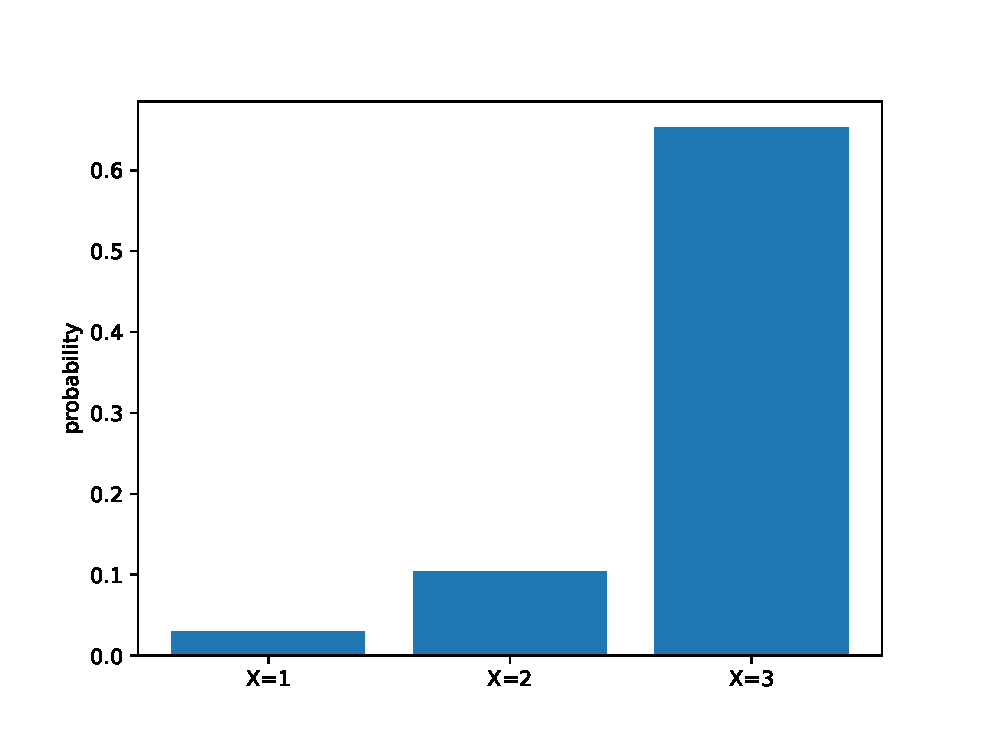
\includegraphics[width=\columnwidth]{./figures/probexm/probexm8.eps}
%\caption{probability ofaccident in an year }
%\label{fig:bt2}
%\begin{lstlisting}
%figs/probexm/probexm8.eps
%\end{lstlisting}
%\end{figure}
\end{enumerate}
